\documentclass[a4paper,onecolumn]{report}
\usepackage{caption}
\usepackage{subcaption}
\usepackage{setspace}
\usepackage{amssymb}
\usepackage[fleqn]{amsmath}
\usepackage{cite}
\usepackage{graphicx}
\usepackage{color}
\usepackage{float}
\usepackage[toc,page]{appendix}
\usepackage[nottoc]{tocbibind}
\usepackage{titlesec}
\usepackage{float}
\usepackage{color}
\usepackage{setspace}
\usepackage{comment}
\titleformat{\chapter}{\normalfont\huge}{\thechapter.}{15pt}{\huge}
\renewcommand*{\familydefault}{\sfdefault}
\hyphenpenalty=5000 
\tolerance=1000

\usepackage[a4paper]{geometry}
\voffset=-80pt
\hoffset=0pt
\topmargin = 0pt
\textwidth = 450pt
\textheight = 770pt
\marginparwidth = 10pt
\oddsidemargin = 5pt
\topmargin = 1pt
\graphicspath{ {/images/} }

\setcounter{tocdepth}{2}

\begin{document}

%----------------------------------------------------------------------------------------
%	TITLE SECTION
%----------------------------------------------------------------------------------------

\begin{titlepage}

\newcommand{\HRule}{\rule{\linewidth}{0.5mm}}
\newcommand{\horrule}[1]{\rule{\linewidth}{#1}}

\center % Center everything on the page

\textsc{\small DELFT UNIVERSITY of TECHNOLOGY}\\[2.5cm] % Name of your university/college

\textsc{\LARGE Artificial Neural Networks}\\[0.5cm] % Major heading such as course name

\HRule \\[0.1cm]
\begin{spacing}{1.6}
{ \huge PROJECT REPORT}\\[-0.4cm] % Title of your document
\end{spacing}
\HRule \\[1.5cm]

\begin{minipage}{0.4\textwidth}
\begin{flushleft} \large
\emph{Authors:}\\
Michiel \textsc{Bongaerts\\}
Marjolein \textsc{Nanninga}\\
Tung \textsc{Phan}\\
Maniek \textsc{Santokhi}
\end{flushleft}
\end{minipage}
~
\begin{minipage}{0.4\textwidth}
\begin{flushright} \large
\end{flushright}
\end{minipage}\\[4cm]

{\large \today}\\[3cm]


\vfill

\end{titlepage}

%----------------------------------------------------------------------------------------
%	CONTENT
%----------------------------------------------------------------------------------------

\tableofcontents

\chapter{Introduction}

Mapping the world around us has always been a human endeavour to advance economical output. A better understanding of the places around us makes for more efficient travelling and exploitation of the land. However, it has always been a very slow and tedious process to produce these maps, something technology has not changed just yet.

A new opportunity has arisen with the arrival of satellite imagery and an ever increasing amount of computational power. An opportunity where this mapping can be done automatically so that this tedious and slow job can be processed even more quickly and perhaps more accurately. It is with this in mind we further analyse any possibilities.\\
\\
This paper proposes an update. Now a more straightforward approach has been chosen in which the emphasis lies on the actual Neural Network rather than the conversion of interpreted images to vector graphic maps. The new approach deals with image patches rather than pixels. This document discusses the newly acquired concept with a list of features and the actual implementation details. Also an updated schedule will be presented. 

\chapter{Concept}
Earlier attempts to conceptualise the idea to automate map making resulted in a proposal that too heavily focussed on the actual map creation rather than the classification. For a Neural Network course this was deemed not befitting enough. The plan was also quite far reaching to start with. Thoughts were put into downscaling this ambitious plan. We played around a bit and came up with a new concept which will be discussed in this chapter. Firstly, an impression is given how the end user interacts with our system. This will lay the groundwork for how the Neural Network will be constructed. Secondly through the principles of MoSCoW a flexible requirements list is established. Actual talk about the classification is done in the subsequent chapter.

\section{Impression}

Below in figure \ref{fig:impression} an impression is given of what the end user will interact with and a possible result that might come about from said interaction.\\

\begin{figure}[h!]
    \centering
    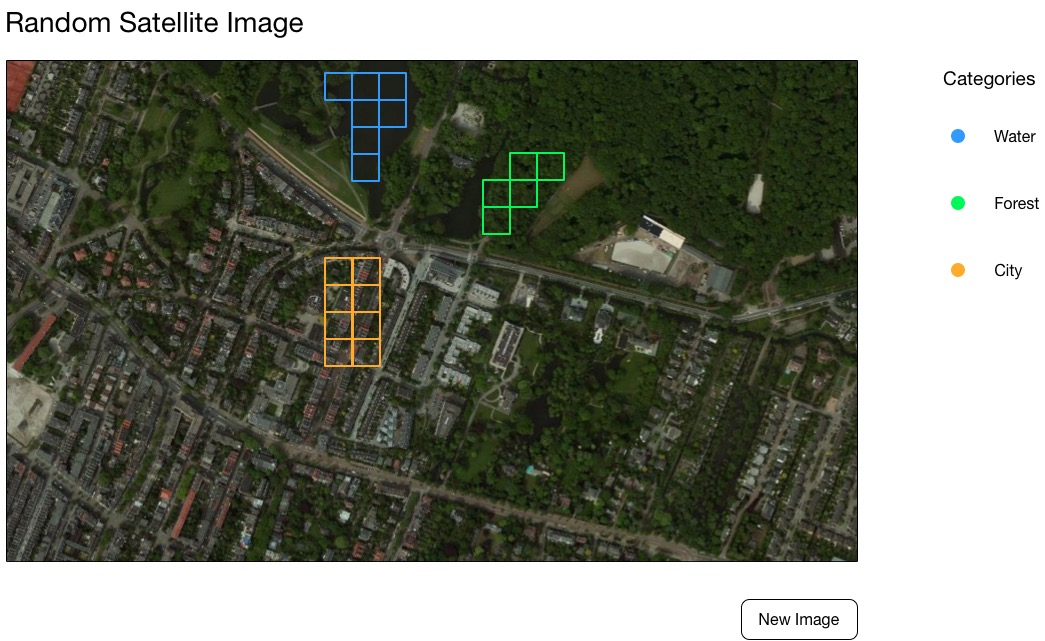
\includegraphics[width=0.8\textwidth]{./images/impression.jpg}
    \caption{Impression of what the user interacts with and a possible outcome.}
	\label{fig:impression}
\end{figure}
\noindent
The most notable attention grabber is the satellite image. This image will be acquired through a random call from a homogenous satellite image database on every new instantiation of the system. Another possibility to acquire new data is by clicking on the 'New image' button. Right of the satellite image one can see labels (Forest, City, Water) which correspond with the labels which are outputs of the classification. Results obtained from our algorithm, given the current satellite image as input, are graphically feed back to the user. The impression above does that by showing a correspondence between image patches and their respective label via color coding laid over the satellite image. This rendition just shows a few islands of resulsts as an example. Normally the entire image will have such arching (which will be a lot more subtle).\\
\\
Figure \ref{fig:grid} shows how it works internally. Two grids are maintained. One with patches the size of 25 by 25 pixels. The other by the size of 50 by 50 pixels. The latter is actually fed to the Neural Network from which will be decided for that patch the percentage of type of label it contains.  Four 50 by 50 pixels will be grouped together to create a square. In the middle the 25 by 25 pixels patch is placed. This patch will eventually be coloured on the satellite image to indicate the type of label. To decide that, a weighted majority vote of the four 50 by 50 pixels surrounding that smaller patch is computed. Like a convolution filter this construction is shifted over the satellite image as to decide for every area on it. As one can imagine, 25 pixels at the borders are omitted. 

\begin{figure}[h!]
    \centering
    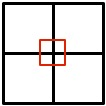
\includegraphics[scale=0.6]{./images/grid.jpg}
    \caption{Grid structure which facilitates the algorithm.}
	\label{fig:grid}
\end{figure}

\section{MoSCoW}
Since a limited amount of time is available and we thought of quite some experiments and features that could be added, we used the MoSCoW method to get our priorities straight and focus on the most important requirements. MoSCow stands for \textit{Must have}, \textit{Should have}, \textit{Could have} and \textit{Would have}. All the requirements are labeled in these four classes.\\

\subsection{Must have}
Must have requirements are critical to project success. 
\begin{itemize}
\item Create code based on a \textit{Convolutional Neural Network} (CNN) that enables automatic classification of patches from satellite images. Considering images acquired on provincial level and a substantial amount of pixels in one patch (at least 50 x 50 pixels). 
\item At least the following classes should be recognized: vegetation, city and water. 
\item Develop a way to visualize the automatic classifications clearly.
\end{itemize}

\subsection{Should have}
Requirements labeled as should have are important to book success, but not necessary for delivery. 

\begin{itemize}
\item Create a clear interface in which the unlabeled images can be uploaded, and the output consists of labeled images. 
\item Calculate the uncertainty in the classification and ask user input for very uncertain patches.
\end{itemize}

\subsection{Could have}
It would be very nice if we would be able to reach the Could have feautures, but they are not critical. 
\begin{itemize}
\item Experiment with pre-processed images (noise reduction, gradient calculations)
\item Analyze images on city level, so with more details present. For this purpose new classes have to be added, such as roadways, cycle paths, 	buildings, distinct vegetations etc. 
\item Experiment with other models than the state-of-the art LeNet-1 CNN. For examples, a CNN in which Genetic Algorithms are incorporated, or implementing an Extreme Learning Machine for the training of the weights. 
\end{itemize}

\subsection{Would have}
These requirements are implemented only in the most ideal situation. They are considered as the dream project, sometimes serving as a suggestion for further projects. 

\begin{itemize}
\item Develop a method for high-detailed automatic vector graphics, in which segmentation of the distinct labeled classes is incorporated.
\item Use the input of the users to improve the automatic classification. 
\item Sell the software package to Google. 
\end{itemize}

\chapter{Implementation}
A plan has been established what kind of application should come about. The previous discussion pressed for a certain kind of structure. One where a Neural Network is central to the problem to be solved. But also a frontend is needed for certain user interaction as well as an infrastructure in the backend which facilitates the communication with said frontend. This chapter discusses these aspects.

\section{Frontend and Backend}
The impression given above in figure \ref{fig:impression} is close to what the end result should look like (although it only displays a certain state). Yet an entire infrastructure outside of the Neural Network is needed to facilitate the application. Below in figure \ref{fig:communication} an infrastructure is visualised via the communication of the two entities.

\begin{figure}[h!]
    \centering
    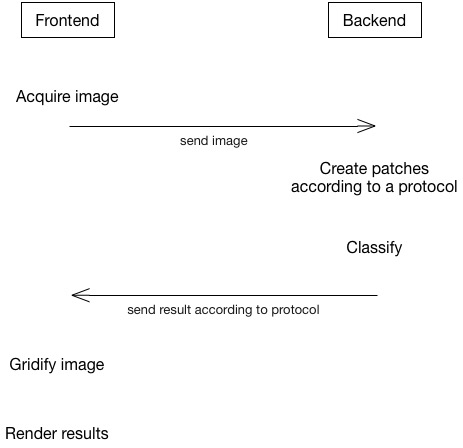
\includegraphics[scale=0.5]{./images/communication.jpg}
    \caption{Communication visualization between frontend and backend.}
	\label{fig:communication}
\end{figure}
\noindent
First, at the frontend, an image is acquired by the user from a database call. The image is immediately send to the backend. There, patches are extracted according to a certain protocol (specific size and sequence). The patches are classified by our Neural Network. Send back to the frontend are the results in a list according to the sequence defined by the protocol. Also a codification of the results is part of the protocol. Back at the frontend the image is made into a grid which corresponds to the size of the protocol. According to the results of the Neural Network these grid windows are coloured.

\section{Dataset}
The image which is being acquired every time comes from the Bing Maps database. A predefined size of the map with satellite view enabled, the labels turned off, no other controls or logos visible and where the hight is 100 meters is put in the frontend.  Randomly a location inside the Netherlands is generated. Now the actual image is taken from the map.

For training, satellite images from the same source and practice mentioned above are drawn on a per category/label basis. Patches are acquired code-wise over those images so that for each patch it is known what category/label belongs to it.


\section{Convolutional Neural Network}
During our research phase, we encountered a variety of papers that describes the use of image classification based on Neural Networks. Most of these papers have one thing in common which is the use of Convolutional Neural Networks (CNN). Since convolution operations are widely used to extract features from images and since these operations can be represented in terms of a Neural Network these properties lead to the existence of the Convolutional Neural Networks. 
\\\\
In general a CNN architecture consist of multiple Convolution layers and sub-sampling layers. It depends on the architecture how these layers are followed by each other. The convolution layer is the layer which results after the convolution operator is performed by the a convolution kernel. Since the gaol is to extract general features from our input image we want the CNN to generalize. This generalization is partly released by dimension reduction. Since convolution operation reduce the dimension of our input map with $\frac{M-N+1}{M}$, where $N$ is the dimension of the convolution kernel and $M$ the dimension of the input map, we want the dimension to be reduced more quickly. This is done by dub-sampling kernels which in general 'squeeze' or average the input map with a certain dimension. This operation is equivalent to a convolution operation but with a larger step-size (convolution uses a stepsize equal to 1) and equal weights for each element in the sub-sampling kernel.

\subsection{LeNet-1}
The model we implement is LeCun's LeNet-1. This model uses an alternating sequence of convolution and sub-sampling layers. The architecture of this network is shown in Figure \ref{fig:Architecture}. The convolution layers act as feauture maps, they consist of a window of a certain size, whose pixels are trainable weights. The sub-sampling layers reduce the dimensionality of the outputs. 
\begin{figure}[h!]
    \centering
    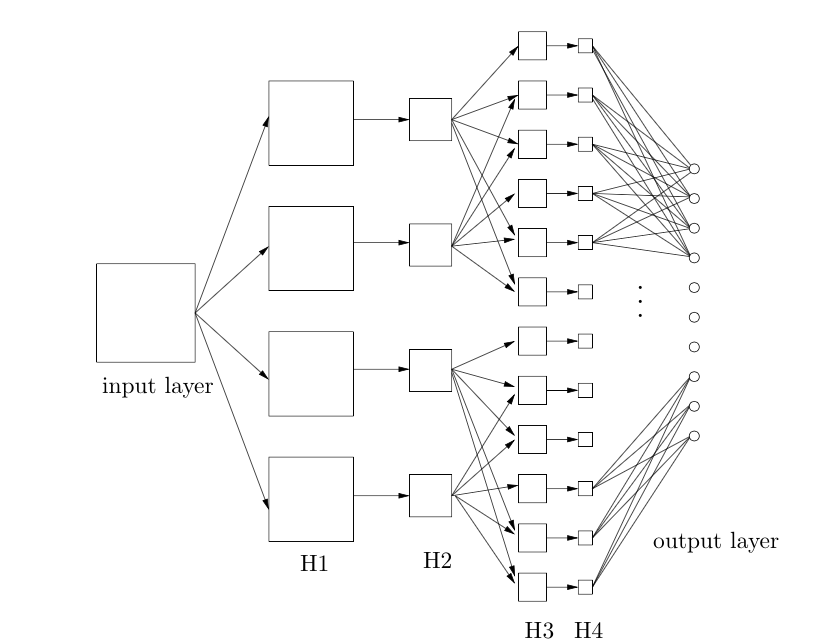
\includegraphics[scale=0.4]{./images/Architecture_CNN.png}
    \caption{The architecture of the CNN proposed by LeNet. H1 and H3 are the convolution layers, H2 and H4 the sub-sampling layers to reduce the dimension. \color{red}{\large{Source:}} }
	\label{fig:Architecture}
\end{figure}
\\\\
One of the biggest advantages of using CNN, and especially LeCun's LeNet-1 implementation, is the incorporation of backpropagation learning. Meaning that all the weights of the layers are adjusted iteratively, eliminating the need to manually create the convolution masks.
\\
\subsection{Back-probabation}



\chapter{Results and Discussion}
In the first phase of our research we made a convolutional neural network based on LeNet-1. We experimented with different convolution kernels in the first layer (H1) of the network and differed the amount of branches in the third layer (H3). We started with manually chosen convolution kernels for both layers H1 and H3. We began with input patches of 50 x 50 followed by a convolution kernel of 5x5 resulting in a feature map of dimensions 46x46. Next, sub-sampling with a dimension reduction of 2 results in a feature map of dimension 23x23. Again we did different 4x4 convolution kernel operation creating branches in H3 resulting in 20x20 feature maps. Sub-sampling with a dimension reduction of 5 resulted in an 4x4 output map. These outputmaps are then connected to two diffent classifcation neurons for Forest and City. \\\\
We used the Sigmoid function as activation function for our classifaction-neurons and performed back-propagation on the weights connecting the output maps with the classification neurons and biases. The first functioning results where found with 4 feature maps in H1 and 2 feature maps in H3 each. We used the convolution kernels shown in figure \ref{fig:firstFilters}. The Network was trained on structure only so no color feautures were included.

\begin{figure}[bth!]
	\centering
	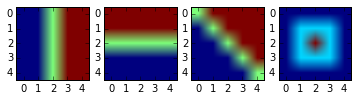
\includegraphics[width=0.5\textwidth]{./images/firstFilters.png}
	\caption{The four filters used in the first stage where the CNN was able to distinguish forest and city.}
	\label{fig:firstFilters}
\end{figure}

In the second phase we tried to extend our classes with \textit{water}.


\begin{figure}[bth!]
	\centering
	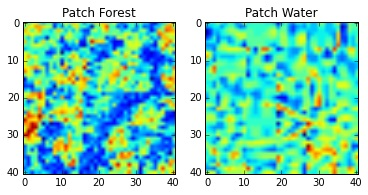
\includegraphics[width=0.5\textwidth]{./images/WaterForestPatch.jpg}
	\caption{A forest and water patch are shown. Their similarity makes it hard for the CNN to distinguish these two classes.}
	\label{fig:WaterForestPatch}
\end{figure}


\chapter{Time schedule}
\begin{center}
  \begin{tabular}{| l | p{5cm}| p{5cm} | r | }
    \hline
    \textbf{Week} & \textbf{Description of work} & \textbf{Deadline} & \textbf{Labour (hours)} \\ \hline \hline
	20 & \begin{itemize} \vspace{-1.75em} \item Implement backpropagation output layer\vspace{-1em}
	\item Start examining how to take into account RGB values \vspace{-1em}
	\item Train on more pictures and examine performance on  other classes like city and water \vspace{-1em}
	\item Start developing frontend/ backend architecture
	\end{itemize}
	& Finish updated proposal & 40 					\\	\hline	
	21 &  \begin{itemize} \vspace{-1.75em} \item Work on implementing communication protocol\vspace{-1em}
	\item Experiments with connecting the nodes of the different layers of the Neural Networks \vspace{-1em}
	\end{itemize}
	& Finish backpropagation output layer, and frontend implementation of the communication protocol& 40 					\\	\hline
	22 & \begin{itemize} \vspace{-1.75em}
	\item In-between overall evaluation \vspace{-1em}
	\item Backend and frontend implementation\vspace{-1em}
	\item Experiment with preprocessed images (noise reduction) \vspace{-1em}
	\item Implement backpropagation further, until layer H3, see Figure \ref{fig:Architecture} \vspace{-1em}
	\end{itemize} & Finish model with complete RGB values and the frontend/backend architecture must be completely finished & 40 					\\  \hline
	23 & Start report writing and implement last adjustments & Finished product for demonstration & 40 	\\	\hline
	24 & Preparation for demo & Demo & 30				\\  \hline
    25 & Project finalization & - & 30 				\\ \hline
    26 & Project finalization & Project report + individual document & 40 \\ \hline
       & & & Total: 468  \\ \hline

    \hline
  \end{tabular}
\end{center}
\end{document}



